% --------------------------------------------------
%  Week 3 – Mathematical Modeling of Disease Spread
%  Focus: Core Theory & Application
%  Version 9 (24 June 2025) - Theory + Case Study
% --------------------------------------------------
\documentclass[14pt,aspectratio=169]{beamer}
\usetheme{Madrid}

% --------------------------------------------------
%         Packages
% --------------------------------------------------
\usepackage{amsmath,amsfonts,amssymb,siunitx}
\usepackage{graphicx}
\usepackage{hyperref}
\usepackage[absolute,overlay]{textpos}
\usepackage{tgtermes} % Use TeX Gyre Termes font
\definecolor{VUblue}{HTML}{002F6C}
\setbeamercolor{alerted text}{fg=VUblue}
\setbeamercolor{structure}{fg=VUblue}
% Graphics path & defaults
\graphicspath{{Figures/}}
\setkeys{Gin}{height=0.45\textheight,keepaspectratio}

% Textpos grid = centimetres (easier positioning)
\setlength{\TPHorizModule}{1cm}
\setlength{\TPVertModule}{1cm}

% --------------------------------------------------
%         Macros
% --------------------------------------------------
\newcommand{\dd}{\,\mathrm{d}}
\newcommand{\RR}{\mathcal{R}_0}
\newcommand{\rinf}{r_\infty}
\newcommand{\sinf}{s_\infty}

% --------------------------------------------------
%         Metadata
% --------------------------------------------------
\title[Modeling Disease Spread]{Advanced SIR Dynamics\\Mathematical Modeling of Disease Spread}
\subtitle{Week 3: Core Theory and Application}
\author{J.~Graham \and T.~Molenaar \and E.~Terjyan}
\setbeamerfont{institute}{size=\footnotesize}
\institute[VU Amsterdam]{%
  Vrije University\\
  of Amsterdam \\
  Dynamical Systems Project}
\date{24 June 2025}

% --------------------------------------------------
\begin{document}

% --------------------------------------------------
% SLIDE 1: Title
% --------------------------------------------------
\begin{frame}[plain]
    \titlepage
\end{frame}

% --------------------------------------------------
% SLIDE 2: Introduction
% --------------------------------------------------
\begin{frame}{Guiding Questions for Today}
    We will develop the core theory of the SIR model and see it in action.
    \begin{enumerate}
        \item \textbf{Invasion:} What is the precise condition for an epidemic to start?
        \item \textbf{Final Size:} How do we calculate the epidemic's total toll?
        \item \textbf{Approximation:} Can we find an analytic solution for the epidemic curve in a critical case?
        \item \textbf{Application:} How can we apply this theory to understand historical epidemic data?
    \end{enumerate}
\end{frame}

% --------------------------------------------------
% SLIDE 3: The Invasion Criterion (Setup)
% --------------------------------------------------
\begin{frame}{The Invasion Criterion: Setup}
    \begin{block}{Question: When can an epidemic start?}
        We analyze the stability of the disease-free equilibrium (DFE).
    \end{block}
    \begin{itemize}
        \item We consider the equation for the infectious proportion, $i$:
        \[ i' = \RR s i - i = (\RR s - 1)i \]
        \item At the start of a potential outbreak, the population is almost entirely susceptible ($s \approx s_0$) and the number of infected is very small ($i \ll 1$).
    \end{itemize}
\end{frame}

% --------------------------------------------------
% SLIDE 4: The Invasion Criterion (Conclusion)
% --------------------------------------------------
\begin{frame}{The Invasion Criterion: Conclusion}
    \begin{itemize}
        \item We can linearize the system around the DFE $(s_0, 0)$. The equation for the small perturbation $i$ becomes:
        \[ \alert{i' \approx (\RR s_0 - 1)i} \]
        \item This implies exponential growth if the coefficient is positive.
    \end{itemize}
    \begin{alertblock}{Invasion Condition}
        An epidemic can occur only if $\RR s_0 > 1$. For a fully susceptible population where $s_0=1$, this gives the classic threshold: $\alert{\RR > 1}$.
    \end{alertblock}
\end{frame}

% --------------------------------------------------
% SLIDE 5: Deriving the Final-Size Relation
% --------------------------------------------------
\begin{frame}{Deriving the Final-Size Relation}
    \begin{block}{Question: What is the total attack rate, $r_\infty$?}
        We find a relationship between the final states by eliminating time.
    \end{block}
    \begin{itemize}
        \item We have the equations for the rates of change:
        \[ s' = -\RR s i \quad \text{and} \quad r' = i \]
        \pause
        \item Using the chain rule, we can write $\frac{\dd r}{\dd s}$:
        \[ \frac{\dd r}{\dd s} = \frac{r'}{s'} = \frac{i}{-\RR s i} = -\frac{1}{\RR s} \]
        \pause
        % \item We integrate this from the start of the epidemic to the end:
        % \[ \int_{r_0}^{r_\infty} \dd r = -\frac{1}{\RR} \int_{s_0}^{s_\infty} \frac{1}{s} \dd s \]
    \end{itemize}
\end{frame}

% --------------------------------------------------
% SLIDE 6: The Final-Size Equation
% --------------------------------------------------
\begin{frame}{The Final-Size Equation}
    \begin{itemize}
        \item We integrate this from the start of the epidemic to the end:
        \[ \int_{r_0}^{r_\infty} \dd r = -\frac{1}{\RR} \int_{s_0}^{s_\infty} \frac{1}{s} \dd s \]
        \item The integration yields the general relation: 
        \[r_\infty - r_0 = -\frac{1}{\RR} \ln\left(\frac{s_\infty}{s_0}\right)\]
    
        \item For an outbreak starting with $(s_0, r_0)=(1, 0)$, and using $s_\infty = 1 - r_\infty$, we get the final implicit equation.
    \end{itemize}
\end{frame}
\begin{frame}{The Final-Size Equation}
    \begin{alertblock}{Canonical Final-Size Equation}
        \[ \alert{1 - r_\infty = e^{-\RR r_\infty}} \]
    \end{alertblock}
    \centering
    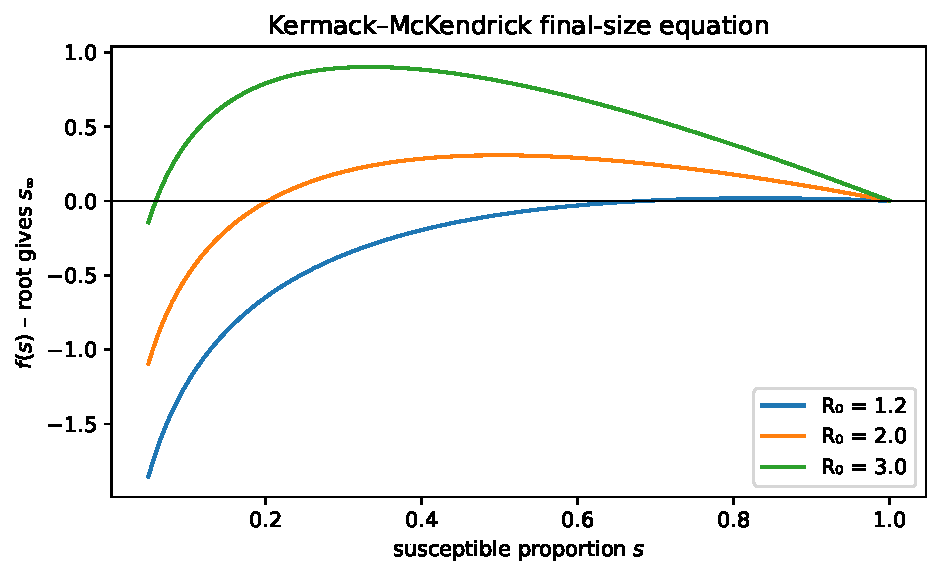
\includegraphics[height=0.4\textheight]{Figures/FinalSizeSketch.pdf}
\end{frame}


% --------------------------------------------------
% SLIDE 7: Near-Threshold Dynamics: The Setup
% --------------------------------------------------
\begin{frame}{Near-Threshold Dynamics: The Setup}
    \begin{block}{Question: Can we find an approximate solution for the epidemic curve?}
        This is possible when $\RR$ is just above 1.
    \end{block}
    \begin{itemize}
        \item \textbf{Step 1: Reduce the system.} Eliminate $s$ and $i$ to get one equation for $r(\tau)$. Since $i=r'$ and $s=1-r-r'$, the equation for $i'$ becomes a single second-order ODE for $r$:
          \[ r'' = \RR(1-r-r')r' - r' \]
    \end{itemize}
    \pause
    \begin{itemize}
        \item \textbf{Step 2: Introduce perturbation.} Let $\RR = 1+\varepsilon$, where $0 < \varepsilon \ll 1$.
    \end{itemize}
\end{frame}

% --------------------------------------------------
% SLIDE 8: Near-Threshold Dynamics: The Approximation
% --------------------------------------------------
\begin{frame}{Near-Threshold Dynamics: The Approximation}
    \begin{itemize}
        \item \textbf{Step 3: Approximate.} We expand the equation for $r''$ and neglect all higher-order terms.
        \item This extensive cancellation simplifies the system dramatically to a famous non-linear ODE.
    \end{itemize}
    \begin{alertblock}{The Riccati Equation for Near-Threshold Dynamics}
    \[ \alert{r'' \approx \varepsilon r' - (r')^2} \]
    This describes the evolution of the cumulative recovered fraction during a "weak" epidemic where $\RR \approx 1$.
    \end{alertblock}
\end{frame}


% --------------------------------------------------
% SLIDE 9: The Near-Threshold Solution
% --------------------------------------------------
\begin{frame}{The Near-Threshold Solution}
    \begin{block}{The Riccati equation has an exact solution.}
        With initial conditions $r(0)=0$ and $r'(0)=i_0$, the solution for the infectious proportion $i(\tau) = r'(\tau)$ is:
    \end{block}
    \[
    \alert{i(\tau) = \frac{\varepsilon\,i_0\,e^{\varepsilon\tau}}{i_0(e^{\varepsilon\tau}-1)+\varepsilon}}
    \]
    \begin{itemize}
        \item This gives us an \textbf{analytic formula} for the entire epidemic wave, providing a powerful tool for analysis and data fitting in the near-threshold regime.
    \end{itemize}
\end{frame}


% --------------------------------------------------
% SLIDE 10: Case Study Application
% --------------------------------------------------
\begin{frame}{Case Study: 1906 Bombay Plague}
    \begin{block}{Application of the Near-Threshold Solution}
        We fit the model for weekly deaths, $D(t) \propto i(t)$, to the historical data.
    \end{block}
    The model to be fitted is derived directly from our analytic solution:
    \[ D(t) = C \cdot i(\gamma t) = C \frac{\varepsilon i_0 e^{\varepsilon \gamma t}}{i_0(e^{\varepsilon \gamma t}-1)+\varepsilon} \]
    % \begin{alertblock}{Fitting Results}
    %     Non-linear least-squares fit gives:
    %     \begin{itemize}
    %         \item $\widehat{\RR} = 1+\widehat{\varepsilon} \approx \alert{1.18}$
    %         \item $\widehat{\gamma} \approx \alert{0.21\; \text{week}^{-1}}$
    %         \item (Mean infectious period $\approx 4.8$ weeks)
    %     \end{itemize}
    % \end{alertblock}
\end{frame}
\begin{frame}{Case Study: 1906 Bombay Plague}

    \begin{alertblock}{Fitting Results}
        Non-linear least-squares fit gives:
        \begin{itemize}
            \item $\widehat{\RR} = 1+\widehat{\varepsilon} \approx \alert{1.18}$
            \item $\widehat{\gamma} \approx \alert{0.21\; \text{week}^{-1}}$
            \item (Mean infectious period $\approx 4.8$ weeks)
        \end{itemize}
    \end{alertblock}
\end{frame}

% --------------------------------------------------
% SLIDE 11: Case Study Insights
% --------------------------------------------------
\begin{frame}{Case Study: Model Insights}
    \begin{block}{The Relationship Between Peak Width and $\RR$}
        The fitting exercise confirms a key qualitative feature of epidemics.
    \end{block}
    \centering
    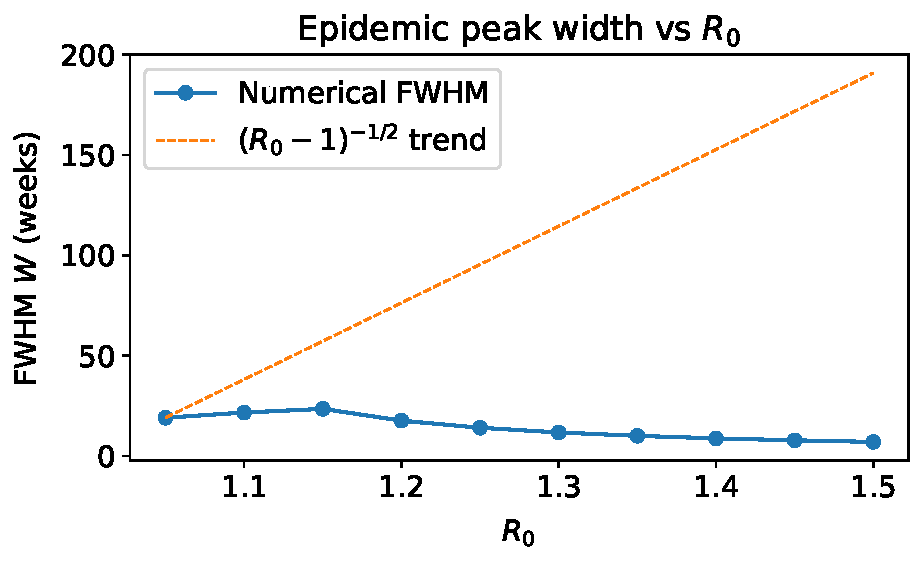
\includegraphics[width=4\linewidth]{Figures/PeakWidth_vs_R0.pdf}
    \vspace{0.7em}
    % The model predicts that epidemics with a higher $\RR$ burn through the population faster, resulting in a \alert{sharper and narrower peak}. Our fit for the Bombay plague, with its low $\RR$ of $1.18$, is consistent with its historically slow and wide epidemic wave.
\end{frame}
\begin{frame}{Case Study: Model Insights}
    % \begin{block}{The Relationship Between Peak Width and $\RR$}
    %     The fitting exercise confirms a key qualitative feature of epidemics.
    % \end{block}
    % \centering
    % 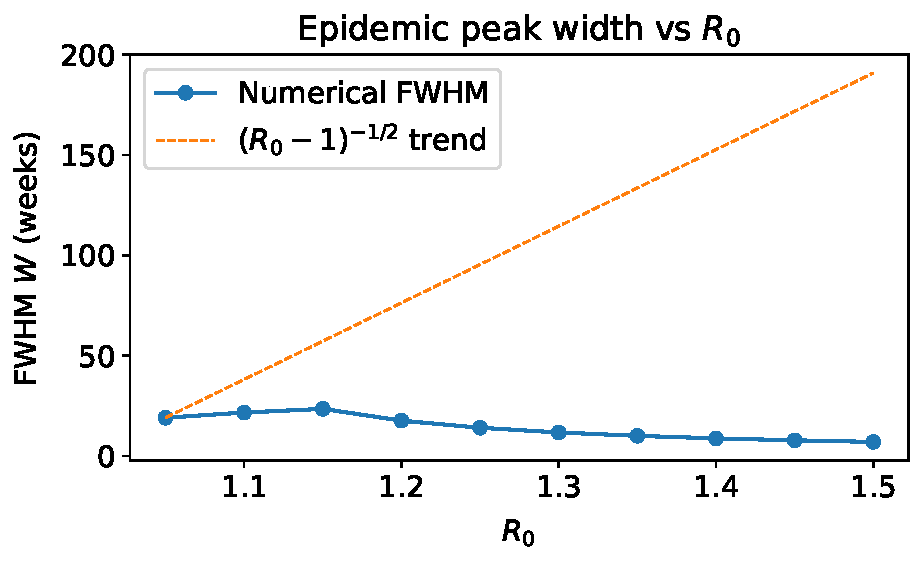
\includegraphics[width=0.8\linewidth]{Figures/PeakWidth_vs_R0.pdf}
    \vspace{0.7em}
    The model predicts that epidemics with a higher $\RR$ burn through the population faster, resulting in a \alert{sharper and narrower peak}. Our fit for the Bombay plague, with its low $\RR$ of $1.18$, is consistent with its historically slow and wide epidemic wave.
\end{frame}

% --------------------------------------------------
% SLIDE 12: Key Take-Aways
% --------------------------------------------------
\begin{frame}{Key Take-Aways}
    \begin{enumerate}
        \item The \alert{Invasion Criterion} ($\RR s_0 > 1$), derived from linear stability analysis, tells us if an epidemic can start.
        \pause
        \item The \alert{Final-Size Equation}, derived by eliminating time, gives us an exact formula for the epidemic's total impact.
        \pause
        \item The \alert{Near-Threshold Approximation} yields an analytic solution for the epidemic curve when $\RR \gtrsim 1$.
        \pause
        \item This theoretical framework can be successfully \alert{applied to historical data} to estimate key epidemiological parameters.
    \end{enumerate}
\end{frame}

% --------------------------------------------------
% SLIDE 13: References
% --------------------------------------------------
\begin{frame}[allowframebreaks]{References}
 % Use text bullets instead of icons
 \setbeamertemplate{bibliography item}[text]
 \footnotesize
 \begin{thebibliography}{99}

    \bibitem[Kermack \& McKendrick(1927)]{Kermack1927}
      Kermack, W.\,O.\ and McKendrick, A.\,G.\
      \newblock A Contribution to the Mathematical Theory of Epidemics. 
      \newblock \emph{Proc.\ Roy.\ Soc.\ A} \textbf{115}, 700–721 (1927).

    \bibitem[Polyanin \& Zaitsev(2002)]{Polyanin2002}
      Polyanin, A.\,D.\ and Zaitsev, V.\,F.\
      \newblock \emph{Handbook of Exact Solutions for Ordinary Differential Equations}. 
      \newblock 2nd ed., Chapman \& Hall/CRC (2002).

 \end{thebibliography}
\end{frame}

% --------------------------------------------------
% SLIDE 14: Closing
% --------------------------------------------------
\begin{frame}[plain]
    \vfill
    \centering{\Huge Thank you!}
    \vfill
    All code and \LaTeX\ at:\ \href{https://github.com/ernestterjyan/mathematical_model_DS}{github.com/ernestterjyan/mathematical\_model\_DS}
    \vfill
\end{frame}

\end{document}